\section{Méthodologie}
\label{sec:methodologie}

Nous présentons ici le déroulement de nos expérimentations qui consistent à étudier le phénomène du renommage et son impact sur le calcul des métriques de procédés. L’objectif étant d’évaluer si le renommage peut biaiser de manière significative les valeurs des métriques de procédés. Pour atteindre cet objectif, nous réalisons deux expérimentations successives.

Le but de la première expérience et de calculer la quantité de renommage durant les périodes de développement des logiciels. S’appuyant sur cette première expérience, notre deuxième expérience fournit une analyse de l’impact du renommage sur les métriques de procédés dans le pire des cas. 

Mais tout d'abord, nous avons besoin d'un ensemble de logiciels afin de former un coprus sur lequel appliquer nos expérimentations. 

\subsection{Corpus}

Nous avons sélectionné un ensemble de projets sur lesquels effectuer nos expérimentations. Des projets open-source, conséquents et connus de la communauté MSR. Ces projets qui sont présentés \tabref{projects} sont notamment régulièrement utilisés par l'équipe de Génie Logiciel au LaBRI. Ces $5$ projets forment un corpus comprenant différents langages de programmation ainsi qu'un nombre de lignes de code et un nombre de développeurs moyennement élevés à élevés par rapport à l'ensemble des projets open source utilisés couramment par la communauté. Les $5$ projets sont gérés sur Git afin de profiter de son mécanisme de traitement du renommage expliqué précédemment. \\

\begin{table*}[h]
\centering
\small
\begin{tabular}{rllp{1.7cm}c}
\toprule
Project & Main language & Size (LoC) & Number of developers & URL\\
\midrule
Jenkins & Java & 200851 & 454 & \url{github.com/jenkinsci/jenkins} \\
JQuery & JavaScript & 41656 & 223 & \url{github.com/jquery/jquery} \\
PHPUnit & PHP & 21799 & 152 & \url{github.com/sebastianbergmann/phpunit}\\
Pyramid & Python & 38726 & 205 & \url{github.com/Pylons/pyramid} \\
Rails & Ruby & 181002 & 2767 & \url{github.com/rails/rails}\\
\bottomrule
\end{tabular}
\caption{Notre corpus de projets.}
\label{tab:projects}
\end{table*}

Les projets de notre corpus suivent des phases distinctes durant leur cycle de vie. Habituellement une période de développement commence avant qu'une première sortie du logiciel, qu'on appelle \texttt{release}, soit accessible aux utilisateurs, puis cette release est maintenue pendant qu'une autre se prépare et ainsi de suite.

Nous avons ainsi deux phases, les phases de maintenance et les phases de développement. Nous divisons ces phases en périodes. Une période est délimité par deux releases et est composé d'un ensemble de versions successives. Chaque projet contient une période qui commence à la création du logiciel et qui se termine à la première release. On appelle cette période la période initiale. Les autres périodes peuvent être divisées en deux groupes, les périodes de releases majeures et les périodes de release mineures. On distingue les releases majeures des mineures par une augmentation significative du numéro de release. Par exemple $1.9-2.0$ pour Jquery, $3.7-4.0$ pour PHPUnit ou $0.13-1.0$ pour Rails. Usuellement, les périodes majeures contiennent un grand nombre de modifications en comparaison des périodes mineures.\\

Les conventions de nommage des releases sont spécifiques à chaque projet, par exemple:
\begin{itemize}
\item PHPunit: \texttt{3.5.0, 3.6.0} etc.
\item Pyramid: \texttt{1.0, 1.1} etc.
\item Jenkins: \texttt{jenkins-1\_400, jenkins-1\_410} etc.
\item Rails: \texttt{v2.0.0, v2.1.0} etc.
\end{itemize}
Nous avons analysé manuellement les dépôts des projets de notre corpus pour identifier leur releases mineures et majeures.\\

Le schéma \figref{model} permet de visualiser un dépôt Git ``type'', avec la branche master depuis laquelle, en remontant l'historique, on peut accéder au contenu de chaque release de la phase de développement et les branches de maintenance, dont la tête (la dernière version de la branche) n'est pas accessible depuis la branche master, qui composent la phase de maintenance.\\

\begin{figure}[h]
  \centering
  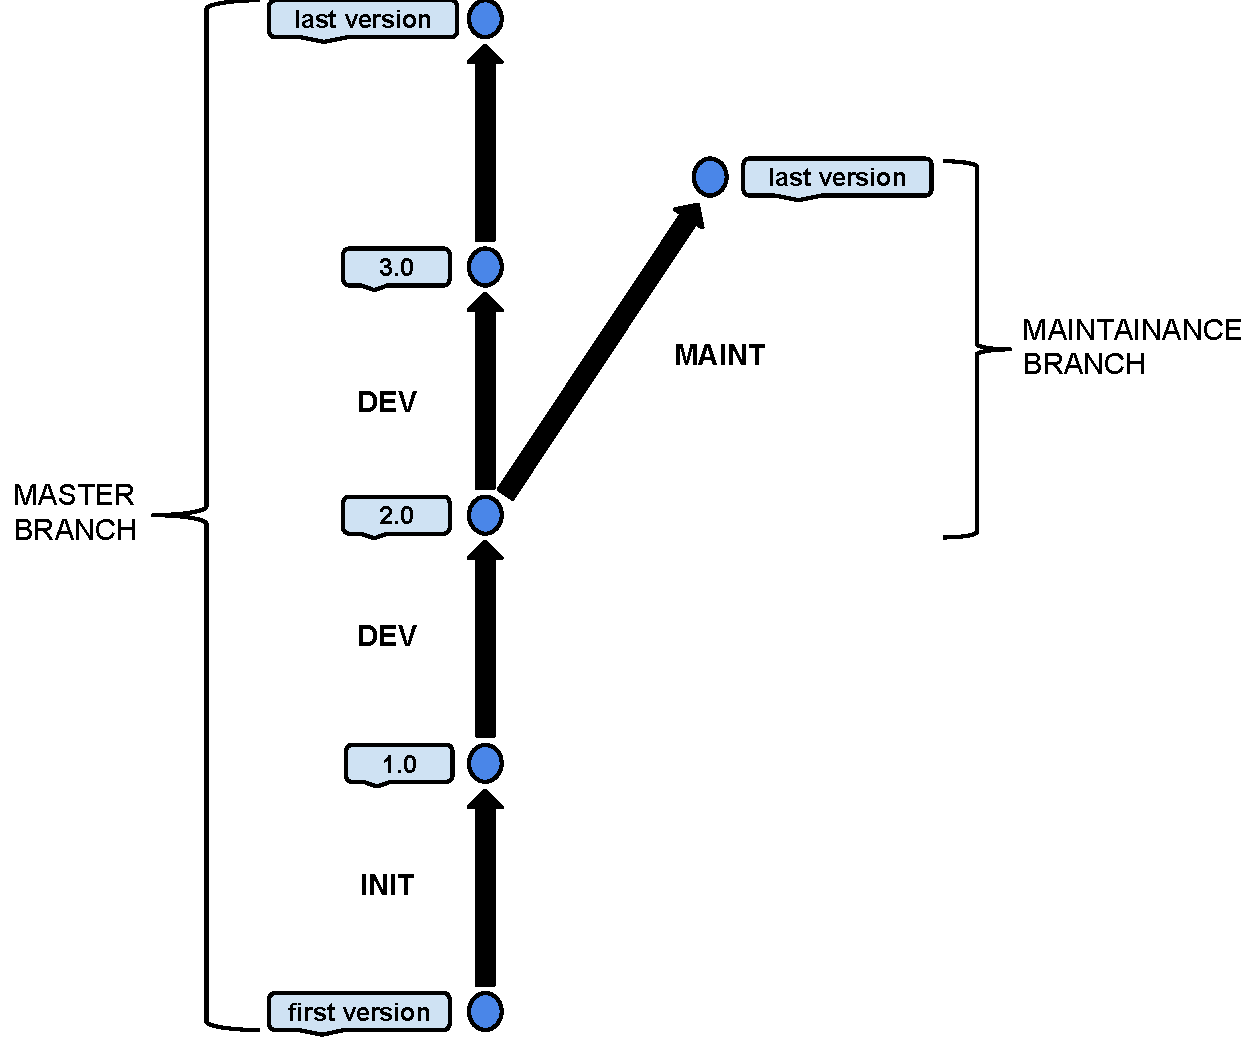
\includegraphics[scale=0.5]{data/figures/periods.pdf}
	\caption{Modèle d'architecture de dépot de code source}
	\label{fig:model}
\end{figure}

De plus, il faut noter que nous avons choisi d'exclure tous les fichiers qui ne sont pas du code source du corpus, étant donné que les métriques de procédés sont habituellement uniquement calculées sur ces fichiers. \\

\subsection{Première expérience}

 L'objectif de notre première expérience est de mieux comprendre le renommage d'entités. Nous souhaitons observer quand les renommages apparaissent et en quelle quantité. Nous avons donc analysé chaque période, comme décrites précédemment, sur chaque projet de notre corpus. 

Pour identifier les renommages, nous comptons sur le mécanisme de Git. Voici la procédure que nous avons suivie :
\begin{enumerate}
\item lister les fichiers existant à la fin de la période.
\item Pour chacun de ces fichiers, extraire sa séquence de modifications durant la période en activant la détection de renommage (commande \texttt{git log -M}).
\item Calculer à partir des informations recueillies le pourcentage de fichiers $\%F_{R}$ qui inclue au moins un renommage dans sa séquence de modification.
\end{enumerate}
\medskip

$\%F_{R}$, calculé sur une période représente en fait le pourcentage de \textbf{l'ensemble} des fichiers du projet qui ont été renommés dans cette période en particulier. $\%F_{R} = \frac{\#AF_{R}}{\#F}$ \\

Nous proposons en complément la même analyse que précédemment, mais en considérant uniquement les fichiers actifs dans cette même période. C'est à dire les fichiers qui ont été modifiés ou créés dans la période. On aura donc le pourcentage de fichiers \textbf{actifs} renommés dans la période : 
$\%AF_{R} = \frac{\#AF_{R}}{\#AF}$. \\
Etant donné que ${\#AF} <= {\#F}$, nous aurons toujours $\%F_{R} <= \%AF_{R}$. Cela nous permet de voir si les périodes qui contiennent le plus de renommage en interne sont aussi celles qui ont un impact sur l'ensemble du projet.\\

À notre connaissance, il n'existe pas d'évaluation empirique de l'algorithme utilisé par Git pour détecter les renommages. Néanmoins, nous procédons à une évaluation manuelle de son comportement dans la Section 4 et nous n'avons pas noté de faux positif sur 100 renommages aléatoires récupérés par notre analyse.\\

\subsection{Deuxième expérience}

L'objectif de la deuxième expérience est de voir si le renommage peut biaiser significativement les valeurs des métriques de procédés décrites ci-dessus. Pour ça, nous effectuons une analyse dans le pire des cas. Nous sélectionnons une période par projet, celle qui a la plus grande valeur de fichiers renommés en excluant la période initiale qui n'est généralement pas observée dans les études. Nous calculons ensuite les trois métriques avec et sans le renommage de fichiers pris en compte. Puis nous calculons la corrélation de coefficient de Spearman entre les métriques avec et sans la détection de renommage. Un coefficient élevé, proche de $1$, indiquera que les métriques avec et sans détection de renommage sont très similaires alors qu'un coefficient plus petit, 0.5 et moins, indiquera que les métriques avec et sans détection de renommage sont très différentes.\\  
